\subsection{Разработка основного окна приложения}

Для разработки основного окна использовались VueJS - основной функционал страницы, less - описание стилей страницы.

Для начала с помощью утилиты vue-cli создался каркас окна приложения. Были созданы минимальные компоненты и связи между ними. На рисунке~\ref{img:vueTemp} представлен изначальный вид vue-приложения.

\begin{figure}[H]
  \centering
  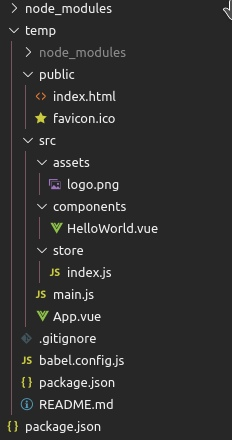
\includegraphics{TexModules/pics/vue_temp.jpg}
  \caption{Шаблон vue-приложения}
  \label{img:vueTemp}
\end{figure}

Здесь в папке public хранятся основной html-документ и логотип приложения. В html-документе производится подключение основного компонента app, указание заголовка и метаданных сайта. На рисунке~\ref{img:htmlTemp} можно увидеть структуру этого html-документа.

\begin{figure}[H]
  \centering
  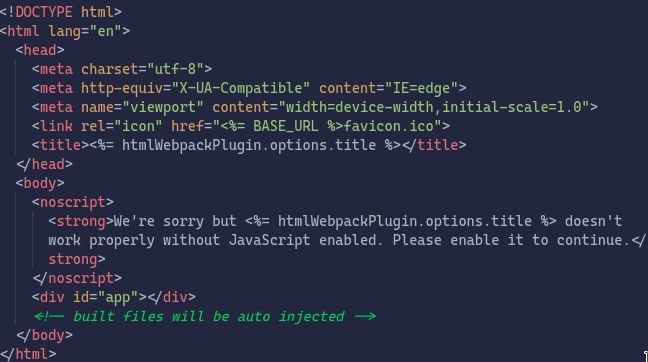
\includegraphics[width=0.95\textwidth]{TexModules/pics/htmlTemp.jpg}
  \caption{Шаблон html-документа}
  \label{img:htmlTemp}
\end{figure}

В папке src находятся компоненты, папка components, файлы js-скриптов, css, изображений, assets, и внутреннего хранилища, store.

Внутренне хранилище представляет собой модуль vuex, в котором можно хранить общие для проекта данные и получать к ним доступ из любой точки программы. Исходный вид vuex-хранилища представлен на рисунке~\ref{img:vuexTemp}.

\begin{figure}[H]
  \centering
  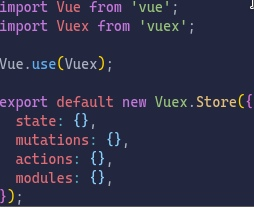
\includegraphics{TexModules/pics/vuexTemp.jpg}
  \caption{Шаблон vuex-хранилища}
  \label{img:vuexTemp}
\end{figure}

В модуле app происходит подключение всех остальных vue-компонентов, находящихся в папке \textbf{src/components}. На рисунке~\ref{img:vueCompTemp} представлена структура vue-компонентов.

\begin{figure}[H]
  \centering
  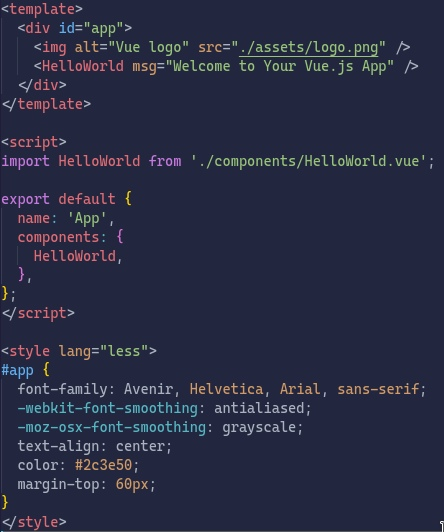
\includegraphics[height=0.4\textheight]{TexModules/pics/vueCompTemp.jpg}
  \caption{Шаблон vue-компонента}
  \label{img:vueCompTemp}
\end{figure}

\subsubsection{Основные моменты разработки}

Окно представляет собой массив полей для ввода текста, позади которых располагаются элементы, которые указывают на то, какие слова были введены неправильно, индикация - красный фон, при наведении указываются варианты замены.

Для текстовых полей были разработаны методы получения списка слов, разделителей слов, методы для объединения строк и создания новых. Также были добавлены функции определения схожести слов с помощью функций помощников.

Были разработаны как синхронные - когда не требуется загрузка больших объемов данных в приложение, так и асинхронные - когда загрузка больших объёмов данных необходима, методы. Пример синхронного метода - поиск по словарю схожих слов; пример асинхронного метода - загрузка словаря в приложение.

Листинги основных файлов можно увидеть в приложении~\ref{sec:e}.